\documentclass{article}\usepackage[]{graphicx}\usepackage[]{xcolor}
% maxwidth is the original width if it is less than linewidth
% otherwise use linewidth (to make sure the graphics do not exceed the margin)
\makeatletter
\def\maxwidth{ %
  \ifdim\Gin@nat@width>\linewidth
    \linewidth
  \else
    \Gin@nat@width
  \fi
}
\makeatother

\definecolor{fgcolor}{rgb}{0.345, 0.345, 0.345}
\newcommand{\hlnum}[1]{\textcolor[rgb]{0.686,0.059,0.569}{#1}}%
\newcommand{\hlstr}[1]{\textcolor[rgb]{0.192,0.494,0.8}{#1}}%
\newcommand{\hlcom}[1]{\textcolor[rgb]{0.678,0.584,0.686}{\textit{#1}}}%
\newcommand{\hlopt}[1]{\textcolor[rgb]{0,0,0}{#1}}%
\newcommand{\hlstd}[1]{\textcolor[rgb]{0.345,0.345,0.345}{#1}}%
\newcommand{\hlkwa}[1]{\textcolor[rgb]{0.161,0.373,0.58}{\textbf{#1}}}%
\newcommand{\hlkwb}[1]{\textcolor[rgb]{0.69,0.353,0.396}{#1}}%
\newcommand{\hlkwc}[1]{\textcolor[rgb]{0.333,0.667,0.333}{#1}}%
\newcommand{\hlkwd}[1]{\textcolor[rgb]{0.737,0.353,0.396}{\textbf{#1}}}%
\let\hlipl\hlkwb

\usepackage{framed}
\makeatletter
\newenvironment{kframe}{%
 \def\at@end@of@kframe{}%
 \ifinner\ifhmode%
  \def\at@end@of@kframe{\end{minipage}}%
  \begin{minipage}{\columnwidth}%
 \fi\fi%
 \def\FrameCommand##1{\hskip\@totalleftmargin \hskip-\fboxsep
 \colorbox{shadecolor}{##1}\hskip-\fboxsep
     % There is no \\@totalrightmargin, so:
     \hskip-\linewidth \hskip-\@totalleftmargin \hskip\columnwidth}%
 \MakeFramed {\advance\hsize-\width
   \@totalleftmargin\z@ \linewidth\hsize
   \@setminipage}}%
 {\par\unskip\endMakeFramed%
 \at@end@of@kframe}
\makeatother

\definecolor{shadecolor}{rgb}{.97, .97, .97}
\definecolor{messagecolor}{rgb}{0, 0, 0}
\definecolor{warningcolor}{rgb}{1, 0, 1}
\definecolor{errorcolor}{rgb}{1, 0, 0}
\newenvironment{knitrout}{}{} % an empty environment to be redefined in TeX

\usepackage{alltt}
\usepackage[utf8]{inputenc}
\usepackage{amsfonts}
\usepackage{tgpagella}
\usepackage{graphicx} % Required for inserting images
\usepackage{polski}
\renewcommand*{\figurename}{Rysunek}
\usepackage{nicefrac, xfrac}
\usepackage[margin=1in]{geometry}
\usepackage{hyperref}
\usepackage{xcolor}
\usepackage{amssymb}
\usepackage[bottom]{footmisc}
\usepackage{float}
\IfFileExists{upquote.sty}{\usepackage{upquote}}{}
\begin{document}



\section{Odsetek naprawianych marek pojazdów}
%Odsetek naprawianych marek pojazdów.

Przeprowadzono analizę, aby sprawdzić jakich marek pojazdy najczęściej pojawiają się w warsztacie do naprawy. 



Można przedstawić procentowy udział marek pojazdów klientów salonu, zaczynając od najczęściej się pojawiającej:

\begin{verbatim}
1. Volkswagen: 13.61%
2. Opel: 11.11%
3. Ford: 8.39%
4. Renault: 5.9%
5. Audi: 5.9%
6. Skoda: 4.76%
7. Hyundai: 4.76%
8. Fiat: 4.54%
9. Bajaj: 4.08%
10. Mercedes-Benz: 3.63%
11. SEAT: 2.95%
12. Citroen: 2.95%
13. BMW: 2.95%
14. Honda: 2.49%
15. Suzuki: 2.27%
16. Kia: 2.27%
17. Peugeot: 2.04%
18. Nissan: 2.04%
19. Mazda: 1.81%
20. Yamaha: 1.59%
21. Toyota: 1.36%
22. TVS: 1.36%
23. Hero: 1.36%
24. Volvo: 1.13%
25. Mitsubishi: 0.91%
26. Porsche: 0.68%
27. Dacia: 0.68%
28. Royal: 0.45%
29. Dodge: 0.23%
30. SsangYong: 0.23%
31. Chevrolet: 0.23%
32. Jeep: 0.23%
33. Jaguar: 0.23%
34. MINI: 0.23%
35. Vespa: 0.23%
36. Mahindra: 0.23%
37. Microcar: 0.23%
\end{verbatim}

Jak widać, najpopularniejsze są pojazdy marki Volkswagen. Pojazdy tej marki stanowią 13.61\% wszystkich. \\

Najmniej popularne są marki SsangYong, Chevrolet, Jeep, Jaguar, MINI, Vespa, Mahindra, Microcar i Dodge. Każdą z nich reprezentowało 0.23\% pojazdów, które się pojawiły w warsztacie. \\

Ilość pojazdów, które były w warsztacie to \ensuremath{2.1831683\times 10^{-321}}. Było więcej samochodów niż motorów. Różnica między ilością typu pojazdu wynosiła \ensuremath{1.6683168\times 10^{-321}}, a samochodów było \ensuremath{1.9257426\times 10^{-321}}).

Sprawdzono także, jak prezentowałyby się rozkład marek, gdyby brano pod uwagę jedynie samochody



Można przedstawić ranking marek, zaczynając od najczęściej się pojawiającej:

\begin{verbatim}
1. Volkswagen: 15.42%
2. Opel: 12.6%
3. Ford: 9.51%
4. Audi: 6.68%
5. Renault: 6.68%
6. Skoda: 5.4%
7. Hyundai: 5.4%
8. Fiat: 5.14%
9. Mercedes-Benz: 4.11%
10. BMW: 3.34%
11. SEAT: 3.34%
12. Citroen: 3.34%
13. Kia: 2.57%
14. Nissan: 2.31%
15. Peugeot: 2.31%
16. Mazda: 2.06%
17. Suzuki: 1.8%
18. Toyota: 1.54%
19. Volvo: 1.29%
20. Mitsubishi: 1.03%
21. Honda: 0.77%
22. Porsche: 0.77%
23. Dacia: 0.77%
24. MINI: 0.26%
25. Chevrolet: 0.26%
26. SsangYong: 0.26%
27. Jaguar: 0.26%
28. Microcar: 0.26%
29. Dodge: 0.26%
30. Jeep: 0.26%
\end{verbatim}

Wśród aut prym wiedzie Volkswagen, reprezentując  15.42\% naprawianych samochodów. \\

Najmniej było samochodów marek Chevrolet, SsangYong, Jaguar, Microcar, Dodge, Jeep i MINI. Było ich 0.26\% dla każdej. \\

Pozostały do sprawdzenia motory.



Udział procentowy poszczególnych marek wśród nich prezentuje się następująco:

\begin{verbatim}
1. Bajaj: 34.62%
2. Honda: 15.38%
3. Yamaha: 13.46%
4. Hero: 11.54%
5. TVS: 11.54%
6. Suzuki: 5.77%
7. Royal: 3.85%
8. Vespa: 1.92%
9. Mahindra: 1.92%
\end{verbatim}

Wśród nich najczęściej naprawiano motory marki Bajaj. Pojazdy tej marki stanowią 34.62\% wszystkich. \\

Najmniej popularnymi motorami są z kolei modele marek Mahindra i Vespa. W warsztacie było zaledwie 1.92\% motorów każdej z wymienionych marek.

\section{Analiza bilansu}

\subsection{Analiza wydatków na zakup pojazdów}

Sprawdziliśmy, jak wyglądają miesięczne wydatki na zakup pojazdów, które w razie potrzeby warsztat naprawia, a następnie sprzedaje.

\begin{knitrout}
\definecolor{shadecolor}{rgb}{0.969, 0.969, 0.969}\color{fgcolor}\begin{figure}[H]

{\centering 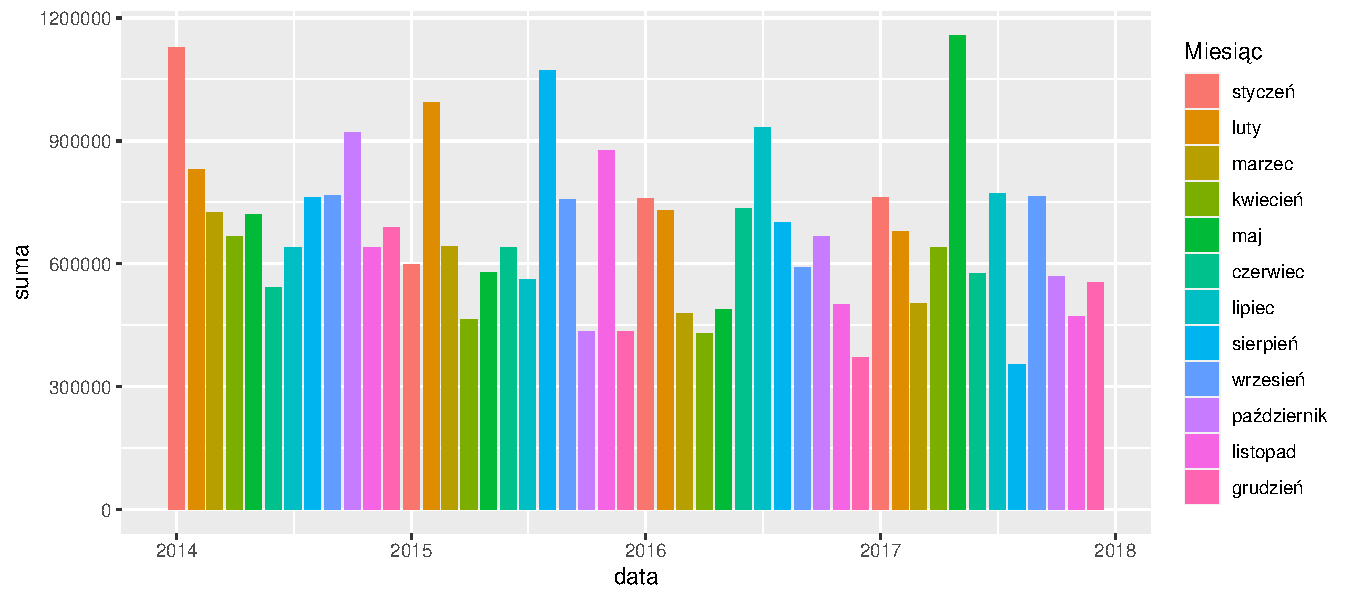
\includegraphics[width=\maxwidth]{figure/fig_zakup_pojazdu-1} 

}

\caption[Miesięczne wydatki na zakup pojazdów]{Miesięczne wydatki na zakup pojazdów}\label{fig:fig_zakup_pojazdu}
\end{figure}

\end{knitrout}

Wykres \ref{fig:fig_zakup_pojazdu} przedstawia miesięczne wydatki na zakup pojazdów. 
Największe wydatki warsztat miał w miesiącu kwiecień 2016. Były one w wysokości 989 tyś. zł. 
Wydatki wielkości 950.8 tyś. zł były drugimi najwyższymi i były 1.04 razy mniejsze od tych największych. Wystąpiły one w miesiącu listopad 2014.
Najmniejsze wydatki warsztat zaobserwował w miesiącu wrzesień 2017 i wyniosły one 400.3 tyś. zł. 
Drugie co do wielkości najniższe wydatki na zakup pojazdów wystąpiły miesiącu luty 2016, a wyniosły one 433.9 tyś. zł.
W każdym miesiącu działania warsztatu wydatki na zakup pojazdów wyniosły przynajmnej 400 tyś. zł.

\subsection{Analiza wydatków na zakup części}

Następnie zostało sprawdzone, jak wyglądają miesięczne wydatki na zakup części potrzebnych do napraw pojazdów.

\begin{knitrout}
\definecolor{shadecolor}{rgb}{0.969, 0.969, 0.969}\color{fgcolor}\begin{figure}[H]

{\centering 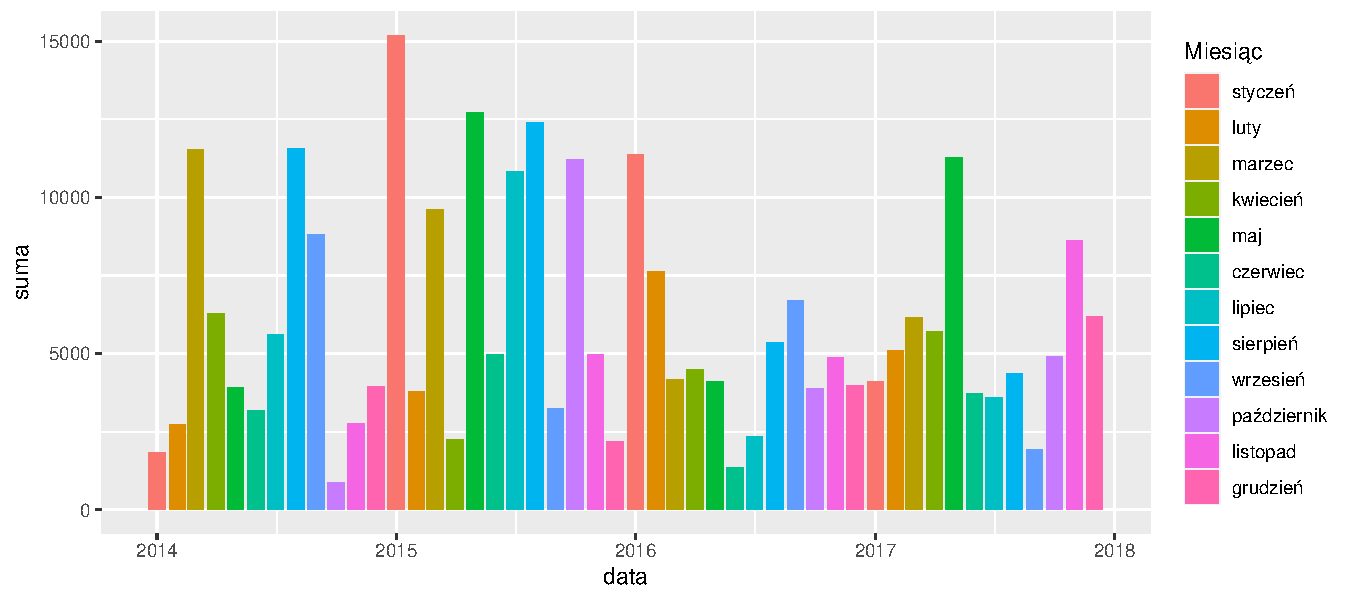
\includegraphics[width=\maxwidth]{figure/fig_zakup_czesci-1} 

}

\caption[Miesięczne wydatki na zakup części]{Miesięczne wydatki na zakup części}\label{fig:fig_zakup_czesci}
\end{figure}

\end{knitrout}

Wykres \ref{fig:fig_zakup_czesci} przedstawia miesięczne wydatki na zakup części do naprawy pojazdów.
Największe wydatki warsztat miał w miesiącu styczeń 2015 i wyniosły one 15.2 tyś. zł. 
Drugie najwyższye wydatkami były wielkości 12.73 tyś. zł i były 1.19 razy mniejsze od tych największych. Wystąpiły one w miesiącu maj 2015.
Najmniejsze wydatki na części zostały odnotowane w miesiącu październik 2014 i wyniosły 0.87 tyś. zł. 
Drugie najmniejsze wydatki wyniosły 1.37 tyś. zł. Wystąpił on w miesiącu czerwiec 2016.
Ogólnie w każdym miesiącu działania warsztatu wydatki na zakup części wyniosły przynajmnej 0.9 tyś. zł.

\subsection{Analiza przychodów z usług warsztatu}

Chcielibyśmy sprawdzić, jak wyglądają miesięczne przychody (lub straty) wynikające z prowadzenia warsztatu. Przez przychód za pojedyńczą usługę uważamy różnicę ceny, którą zapłacił klient i kwoty zapłaconej za części. Przeanaliowane zostaną przychody z uwzględnieniem kosztu własnych napraw oraz bez nich.

\begin{knitrout}
\definecolor{shadecolor}{rgb}{0.969, 0.969, 0.969}\color{fgcolor}\begin{figure}[H]

{\centering 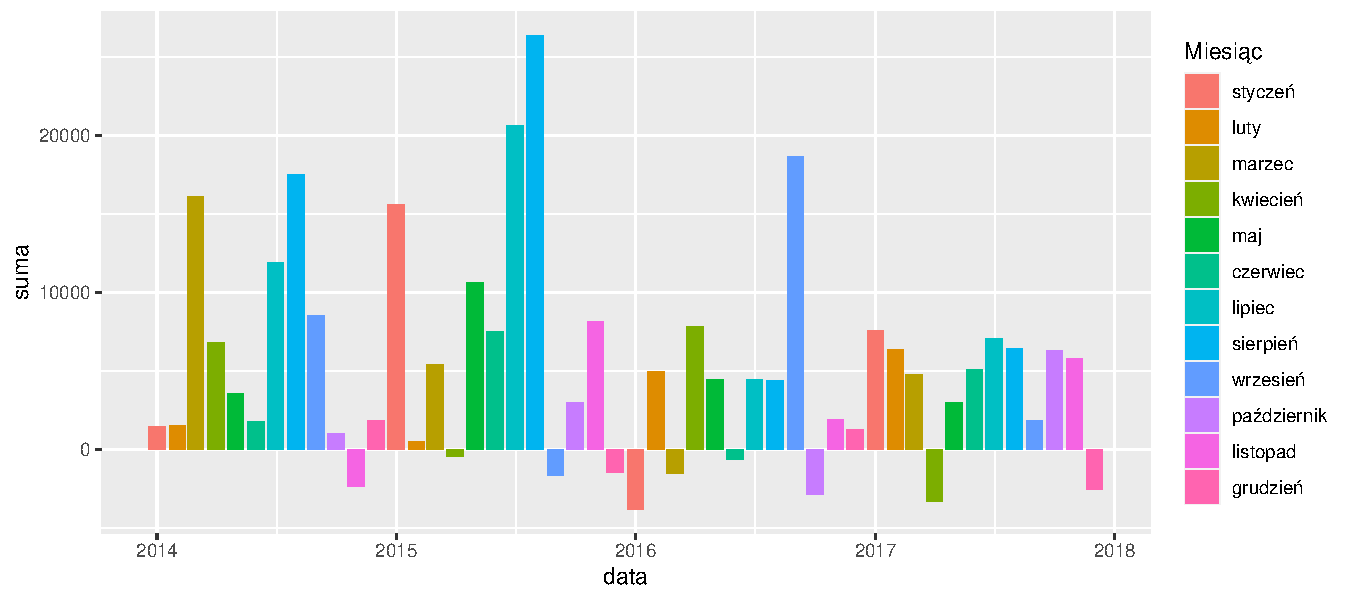
\includegraphics[width=\maxwidth]{figure/fig_uslugi-1} 

}

\caption[Miesięczny przychód wynikający z prowadzenia warsztatu z wliczonymi kosztami napraw własnych]{Miesięczny przychód wynikający z prowadzenia warsztatu z wliczonymi kosztami napraw własnych}\label{fig:fig_uslugi}
\end{figure}

\end{knitrout}

Na wykresie \ref{fig:fig_uslugi} przedstawiony jest miesięczny przychód wynikający z prowadzenia warsztatu. Zostały na nim uwzględnione koszty napraw własnych. 
Największy przychód był zaobserwowany w miesiącu sierpień 2015 i wyniósł on wtedy 26.37 tyś. zł.
Następny co do wielkości przychód wystąpił w miesiącu lipiec 2015, wyniósł on 20.61 tyś. zł. Jest on 1.28 razy mniejszy niż najwyższy przychód.
Najmniejszy przychód warsztat odnotował w miesiącu styczeń 2016, który wyniósł -3.86 tyś. zł. 
Drugi najmniejszy przychód wyniósł -3.34 tyś. zł i wystąpił w miesiącu kwiecień 2017.

\begin{knitrout}
\definecolor{shadecolor}{rgb}{0.969, 0.969, 0.969}\color{fgcolor}\begin{figure}[H]

{\centering 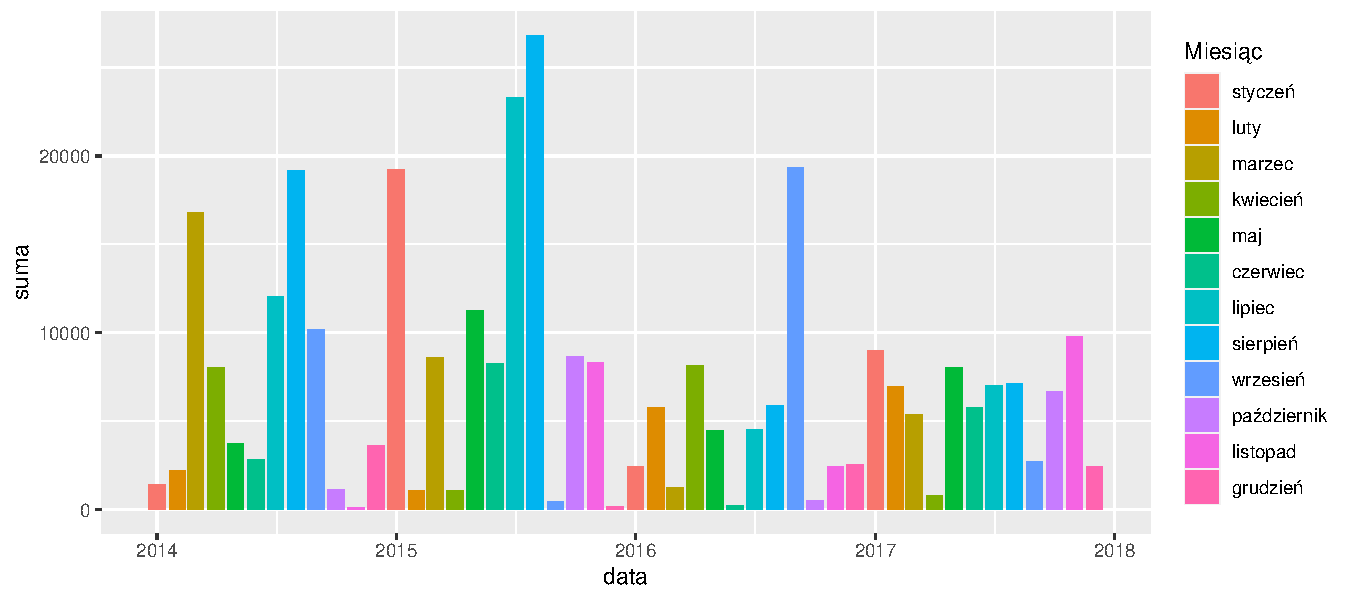
\includegraphics[width=\maxwidth]{figure/fig_uslugi2-1} 

}

\caption[Miesięczny przychód wynikający z prowadzenia warsztatu bez wliczonych kosztów napraw własnych]{Miesięczny przychód wynikający z prowadzenia warsztatu bez wliczonych kosztów napraw własnych}\label{fig:fig_uslugi2}
\end{figure}

\end{knitrout}

Na wykresie \ref{fig:fig_uslugi2} przedstawiony jest miesięczny przychód wynikający z prowadzenia warsztatu, ale tym razem bez uwzględnienia kosztów własnych. 
Największy przychód warsztat zaobserwował w miesiącu sierpień 2015, który wyniósł 26.83 tyś. zł.
Drugi zaś co do wielkości przychód wsytąpił w miesiącu lipiec 2015, wyniósł on 23.29 tyś. zł, czyli jest 1.15 razy mniejszy niż ten najwyższy zaobserwowany.
Najmniejszy przychód został odnotowany w miesiącu listopad 2014 i wyniósł 0.15 tyś. zł. 
Drugi najmniejszy przychód wyniósł 0.21 tyś. zł. Wystąpił on w miesiącu grudzień 2015.

\subsection{Koszty wypłat dla pracowników}

\begin{knitrout}
\definecolor{shadecolor}{rgb}{0.969, 0.969, 0.969}\color{fgcolor}

{\centering 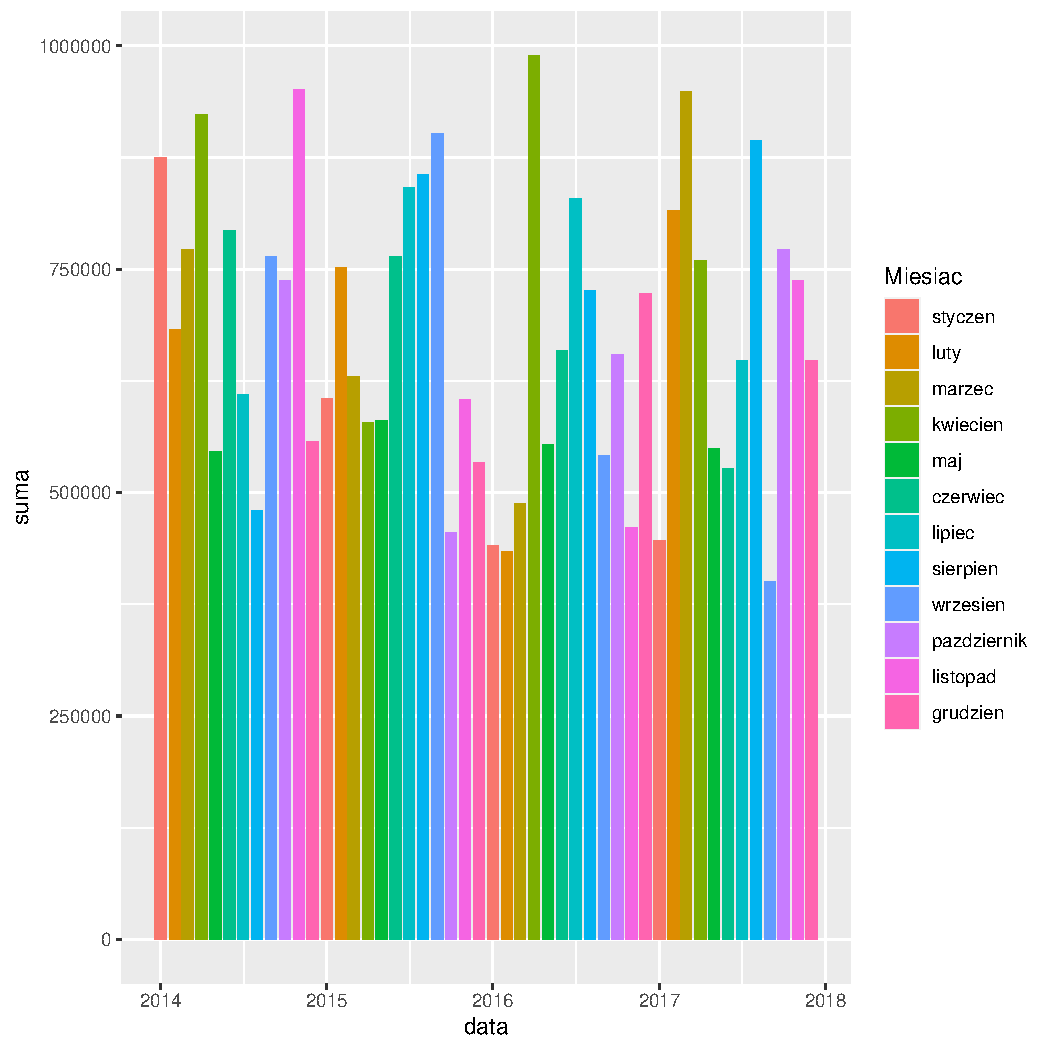
\includegraphics[width=\maxwidth]{figure/unnamed-chunk-5-1} 

}


\end{knitrout}

Zakładamy, że płaca w miesiącu to 160*płaca (przy zatrudnieniu/zwolnieniu pracownika patrze ile dni w miesiacu pracownik pracowal i robie ulamek, np. jak zatrudnili go 3 marca to dostaje round(płaca*160*29/31,2)) i podobnie ostatni to by byl round(płaca*160*3/31,2), wypłacamy pieniądze 1 dnia kolejnego miesiąca (np za styczeń wypłacamy 1 lutego)

{\color{red} To opisz proszę}

\subsection{Samochody wpływy}

\begin{knitrout}
\definecolor{shadecolor}{rgb}{0.969, 0.969, 0.969}\color{fgcolor}

{\centering 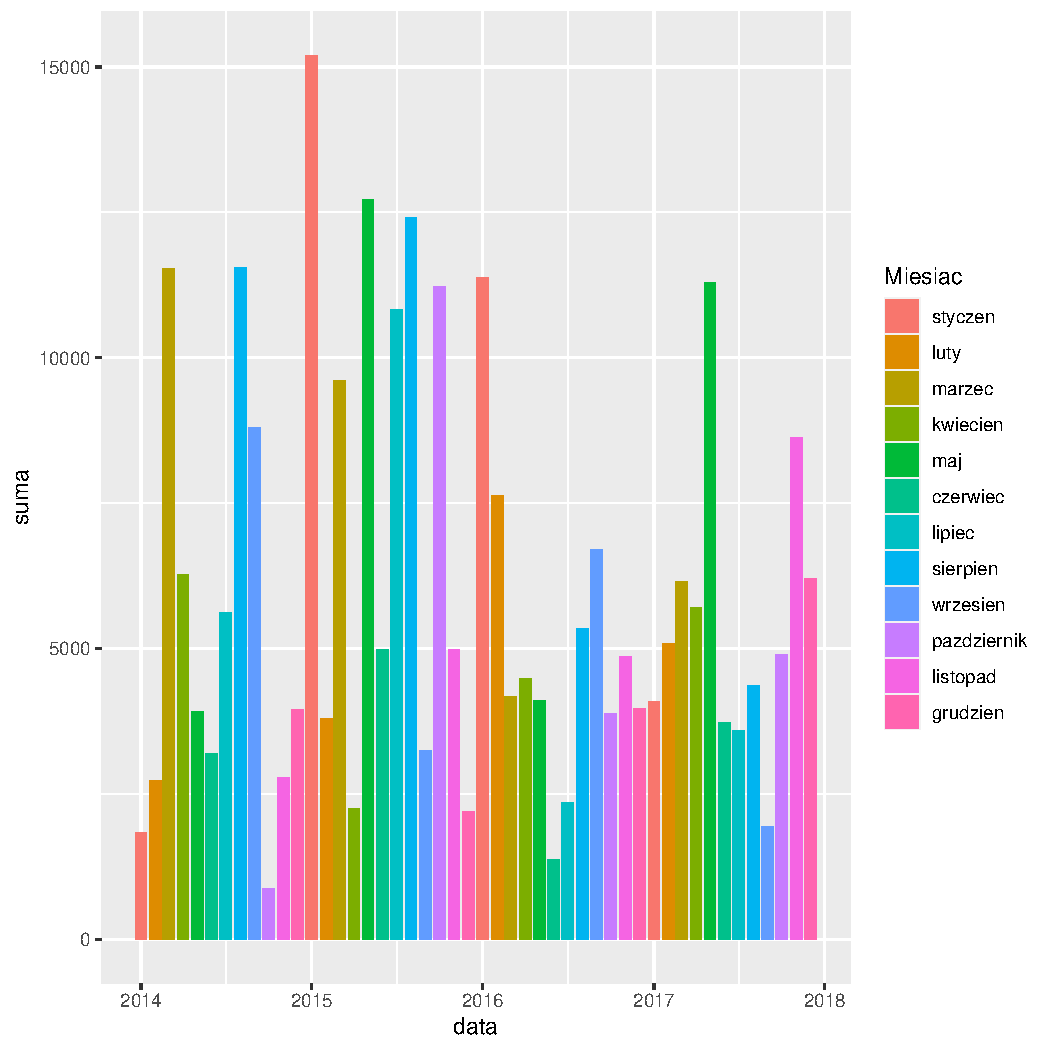
\includegraphics[width=\maxwidth]{figure/unnamed-chunk-6-1} 

}


\end{knitrout}


Jak są wpłaty to robimy dla wszystkich oprócz ostatniej floor z dzielenia, a ostatnia to cena zakupu - te raty co juz splacono
{\color{red} to do opisu}

\subsection{Bilans miesięczny}


\begin{knitrout}
\definecolor{shadecolor}{rgb}{0.969, 0.969, 0.969}\color{fgcolor}

{\centering 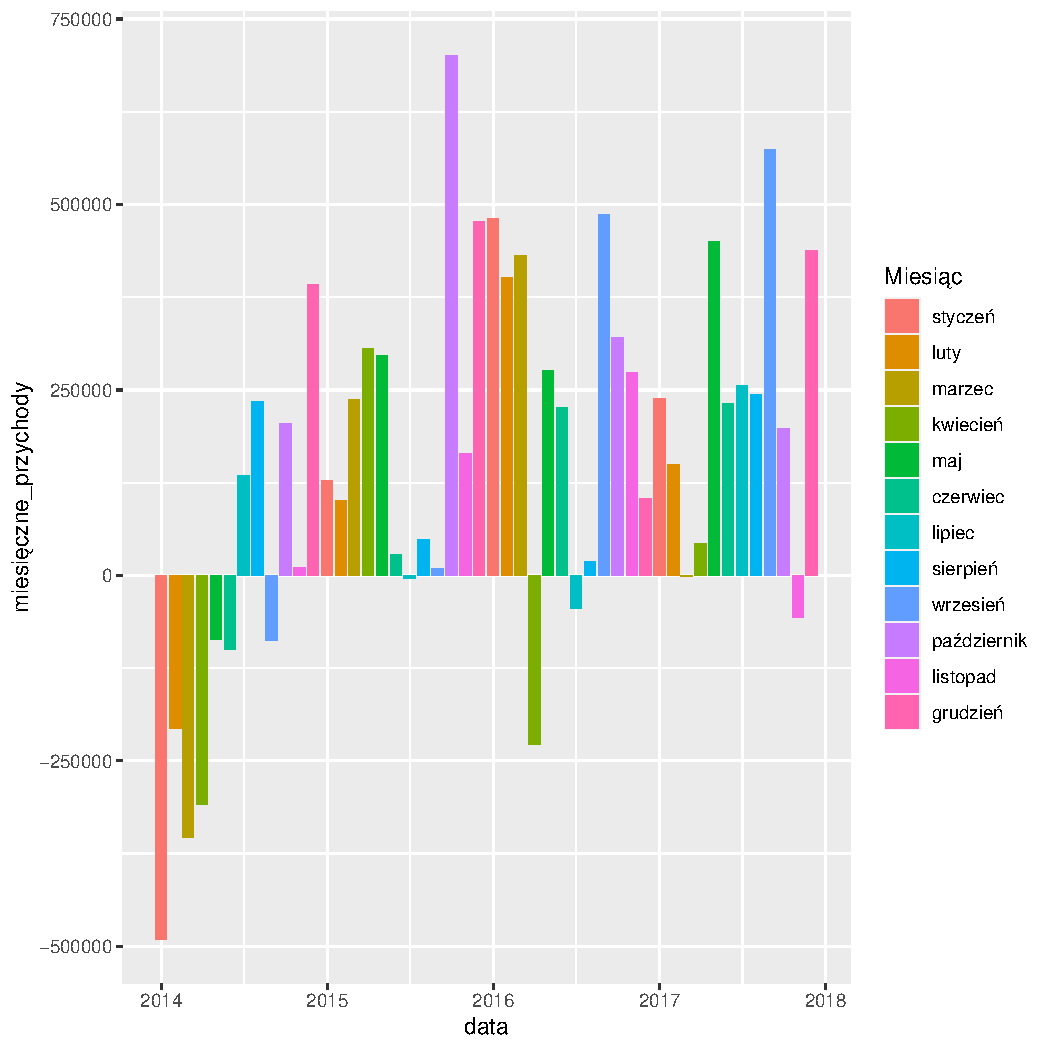
\includegraphics[width=\maxwidth]{figure/unnamed-chunk-7-1} 

}


\end{knitrout}

złączenie: na miesiąc = naprawy(te z minusami, bo mają razem części) + sprzedaż pojazdu -zakup pojazdu - wypłaty (czy ja coś pominęłam?)

\begin{knitrout}
\definecolor{shadecolor}{rgb}{0.969, 0.969, 0.969}\color{fgcolor}

{\centering 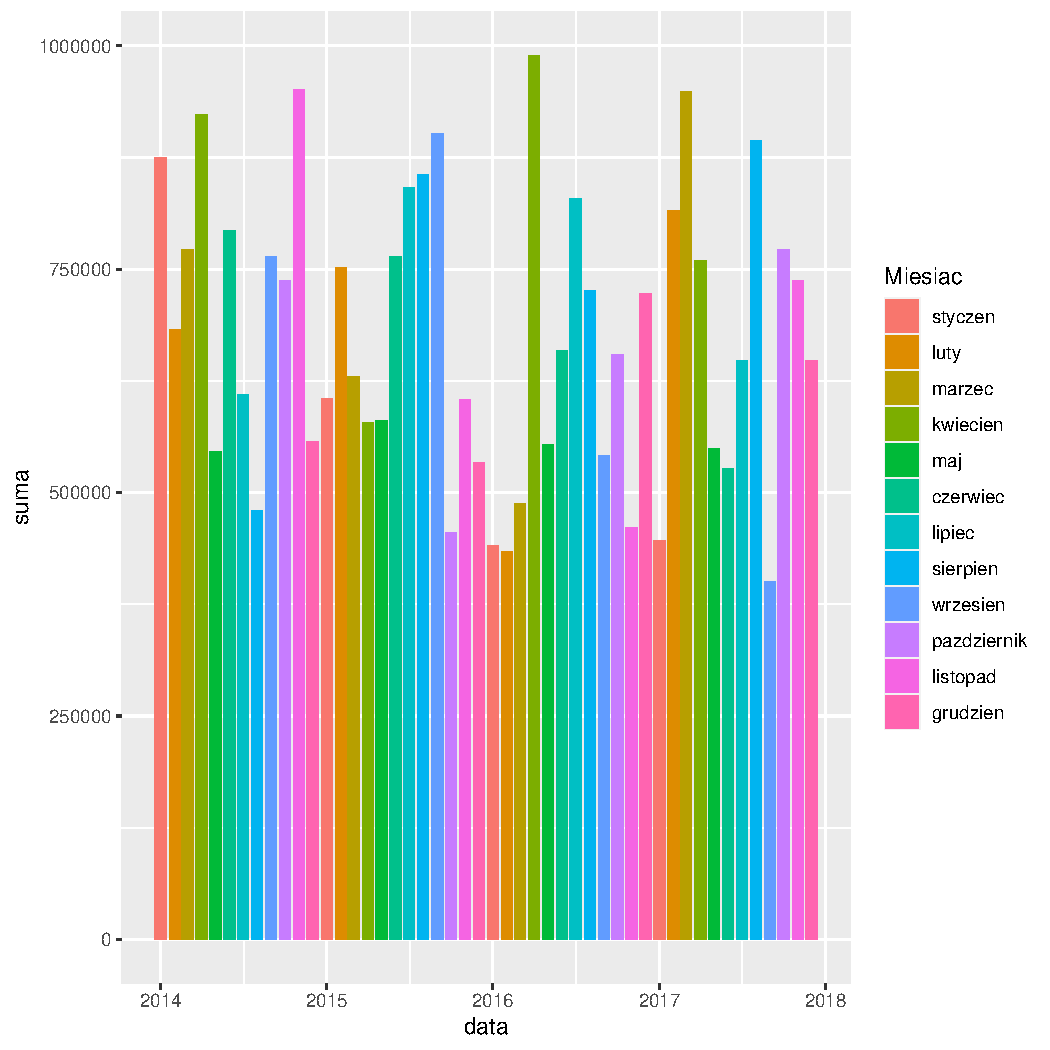
\includegraphics[width=\maxwidth]{figure/unnamed-chunk-8-1} 

}


\end{knitrout}

{\color{red} to też do opisu}


\section{Kim są najlepszy mechanik i sprzedawca w warsztacie?}

Przez czas działania warsztatu „Pimp My Wheels” osoba zarządzająca warsztatem nie była skłonna do dawania podwyżek, jednak postanowiła zlecić informatykowi by przeanalizował bazę danych i znalazł pracowników, którzy zasługują na większe wynagrodzenie. \\

Warsztatowi zależy na tym by sprzedawca zarobił dla firmy dużą kwotę (Może to osiągnąć sprzedając bardzo dużo pojazdów albo sprzedając wartościowe pojazdy), ale także by był charyzmatyczny i był w stanie przekonać wiele osób do zakupu. Rozważone wobec tego zostanie to który obecnie pracujący sprzedawca przekonał klientów do kupna największej liczby pojazdów, a który odpowiada za najwięcej środków pochodzących ze sprzedaży. \\


Tabela, w której są dane o sprzedawcach  pracujących w dowolnym momencie w warsztacie wygląda następująco:

\begin{knitrout}
\definecolor{shadecolor}{rgb}{0.969, 0.969, 0.969}\color{fgcolor}\begin{kframe}
\begin{verbatim}
##        sprzedawca     suma ile_sprzedanych płaca id_pracownika status
## 1 Dorota Drewniak 19783751             360  53.8             3      1
## 2  Janusz Kończal 25277133             413  59.5             2      0
\end{verbatim}
\end{kframe}
\end{knitrout}

Jeżeli pracownik odszedł z warsztatu, to nielogicznym jest, by rozważać danie mu podwyżki.

Po usunięciu pracowników, którzy już nie pracują otrzymujemy taką tabelę:

\begin{knitrout}
\definecolor{shadecolor}{rgb}{0.969, 0.969, 0.969}\color{fgcolor}\begin{kframe}
\begin{verbatim}
##        sprzedawca     suma ile_sprzedanych płaca id_pracownika status
## 1 Dorota Drewniak 19783751             360  53.8             3      1
\end{verbatim}
\end{kframe}
\end{knitrout}

Obecnie tylko jedna osoba pracuje w firmie na tym stanowisku i jest to Dorota Drewniak. Ta osoba sprzedała pojazdy łącznie na kwotę wynoszącą łącznie 19783750.86 zł na sprzedaży pojazdów, co stanowi 87.81\% średniej sumy całej kwoty, którą wynegocjował z klientami sprzedawca przez cały okres pracy. Zarabiana przez tego pracownika kwota za godzinę pracy (53.80 zł) stanowi 94.97 \% średniej płacy sprzedawcy (56.65 zł). Różnica procentowa wynosi 7.16\% na korzyść pracownika, jednak biorąc pod uwagę, że to jedyna osoba pracująca obecnie jako sprzedawca w warsztacie i była porównywana z byłymi pracownikami, można jej zaoferować podniesienie płacy, by pozytywnie wpłynąć na jej motywację. \\

Ten sprzedawca namówił klientów do kupna 360 pojazdów, co stanowi 93.26\% ilości sprzedanych pojazdów dzielonej przez liczbę kiedykolwiek zatrudnionych pracowników. Podobnie jak wcześniej, możemy spróbować porównać zarobki z ilością sprzedaży. różnica między stosunkiem zarobków do średniej płacy i sprzedanych przez obecnego sprzedawcę samochodów do średniej liczby przypadającej na sprzedawcę  wynosi 1.70\%. Gdyby jedynie brać pod uwagę ilość sprzedaży przy analizie to możnaby było zauważyć, że różnica jest na korzyść pracownika. Drobna podwyżka może jednak okazać się dla niego dobrym motywatorem. 

\begin{knitrout}
\definecolor{shadecolor}{rgb}{0.969, 0.969, 0.969}\color{fgcolor}\begin{kframe}
\begin{verbatim}
##         mechanik   suma ile_napraw płaca id_pracownika status
## 1 Wojciech Raźny  85264        214  59.1             6      0
## 2  Dariusz Kuraś 120170        253  45.4             7      1
## 3  Józef Stępień 122724        207  53.0             4      1
\end{verbatim}
\end{kframe}
\end{knitrout}


Tutaj również należy usunąć z tabeli mechaników, którzy już nie pracują w warsztacie. \\

Pozostali następujący pracownicy:

\begin{knitrout}
\definecolor{shadecolor}{rgb}{0.969, 0.969, 0.969}\color{fgcolor}\begin{kframe}
\begin{verbatim}
##        mechanik   suma ile_napraw płaca id_pracownika status
## 1 Dariusz Kuraś 120170        253  45.4             7      1
## 2 Józef Stępień 122724        207  53.0             4      1
\end{verbatim}
\end{kframe}
\end{knitrout}

Mechanik, który wykonał w firmie naprawy, za które klienci (po odliczeniu kosztu części) zapłacili najwięcej to Józef Stępień i jest to kwota 122724.00 zł, co stanowi 112.19\% średniego zysku z napraw na mechanika. Pracownik zarabia kwotę 53.00 zł za godzinę pracy, co stanowi 100.95 \% średniej płacy mechanika (52.50 zł). Różnica między tymi wartościami to 11.24\%, wobec czego dobrze by było, gdyby firma zauważyła świetne wyniki tego pracownika i jego pozytywny wpływ na finanse warsztatu. \\

Pracownik, który dokonał największej liczby napraw to Dariusz Kuraś. . Liczba napraw dokonana przez niego wynosi 253, co stanowi 112.95\% średniej ilości napraw na mechanika. Jej zarobki wynoszą 45.40 zł na godzinę, co stanowi 86.48 \% średniej płacy mechanika (52.50 zł). Różnica między tymi dwoma wartościami wynosi 26.47\%, więc podwyżka wydaje się rozsądnym rozwiązaniem, aby okazać mechanikowi, że warsztat go docenia.



\end{document}
